

\tikzset{every picture/.style={line width=0.75pt}} %set default line width to 0.75pt        

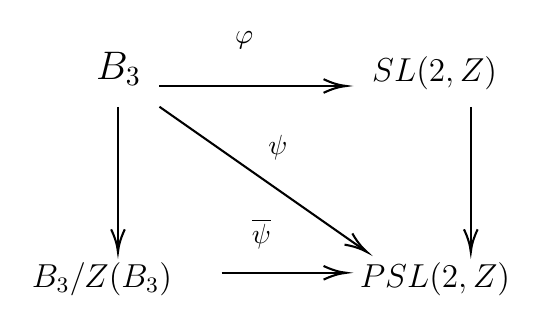
\begin{tikzpicture}[x=0.75pt,y=0.75pt,yscale=-1,xscale=1]
%uncomment if require: \path (0,877); %set diagram left start at 0, and has height of 877

%Straight Lines [id:da11668079361738581] 
\draw    (210,120) -- (298,120) ;
\draw [shift={(300,120)}, rotate = 180] [color={rgb, 255:red, 0; green, 0; blue, 0 }  ][line width=0.75]    (10.93,-3.29) .. controls (6.95,-1.4) and (3.31,-0.3) .. (0,0) .. controls (3.31,0.3) and (6.95,1.4) .. (10.93,3.29)   ;
%Straight Lines [id:da060790583995789405] 
\draw    (360,130) -- (360,198) ;
\draw [shift={(360,200)}, rotate = 270] [color={rgb, 255:red, 0; green, 0; blue, 0 }  ][line width=0.75]    (10.93,-3.29) .. controls (6.95,-1.4) and (3.31,-0.3) .. (0,0) .. controls (3.31,0.3) and (6.95,1.4) .. (10.93,3.29)   ;
%Straight Lines [id:da8757010499358835] 
\draw    (210,130) -- (308.36,198.85) ;
\draw [shift={(310,200)}, rotate = 214.99] [color={rgb, 255:red, 0; green, 0; blue, 0 }  ][line width=0.75]    (10.93,-3.29) .. controls (6.95,-1.4) and (3.31,-0.3) .. (0,0) .. controls (3.31,0.3) and (6.95,1.4) .. (10.93,3.29)   ;
%Straight Lines [id:da8152415293734984] 
\draw    (240,210) -- (298,210) ;
\draw [shift={(300,210)}, rotate = 180] [color={rgb, 255:red, 0; green, 0; blue, 0 }  ][line width=0.75]    (10.93,-3.29) .. controls (6.95,-1.4) and (3.31,-0.3) .. (0,0) .. controls (3.31,0.3) and (6.95,1.4) .. (10.93,3.29)   ;
%Straight Lines [id:da5884397458751206] 
\draw    (190,130) -- (190,198) ;
\draw [shift={(190,200)}, rotate = 270] [color={rgb, 255:red, 0; green, 0; blue, 0 }  ][line width=0.75]    (10.93,-3.29) .. controls (6.95,-1.4) and (3.31,-0.3) .. (0,0) .. controls (3.31,0.3) and (6.95,1.4) .. (10.93,3.29)   ;

% Text Node
\draw (178,102.4) node [anchor=north west][inner sep=0.75pt]  [font=\Large]  {$B_{3}$};
% Text Node
\draw (311,104.4) node [anchor=north west][inner sep=0.75pt]  [font=\large]  {$SL( 2,\mathbb{Z})$};
% Text Node
\draw (305,203.4) node [anchor=north west][inner sep=0.75pt]  [font=\large]  {$PSL( 2,\mathbb{Z})$};
% Text Node
\draw (245,92.4) node [anchor=north west][inner sep=0.75pt]    {$\varphi $};
% Text Node
\draw (261,142.4) node [anchor=north west][inner sep=0.75pt]    {$\psi $};
% Text Node
\draw (253,182.4) node [anchor=north west][inner sep=0.75pt]    {$\overline{\psi }$};
% Text Node
\draw (147,203.4) node [anchor=north west][inner sep=0.75pt]  [font=\large]  {$B_{3} /Z( B_{3})$};


\end{tikzpicture}
